\documentclass[10pt]{article}

\usepackage{amsmath}
\usepackage[colorlinks = true, urlcolor = red, citecolor = blue, linkcolor = red]{hyperref}
\usepackage{fancyhdr}
\usepackage{amssymb}
\usepackage{geometry}
\usepackage{bm}
\usepackage[pdftex]{graphicx}
\usepackage{setspace}
\usepackage{multicol}

\onehalfspacing

\geometry{left=.9in,right=.9in,top=1.1in,bottom=1.1in}

\begin{document}
\thispagestyle{fancy}

\lhead{\Large{\bf{FanDuel - Round One}}}

\subsection*{Methods}

\noindent Winning at FanDuel requires solving the following problem:
\begin{gather}
\label{obj}
\max_{\bm{x}} \; {\bm f} \cdot {\bm X} \\
\label{con}
\text{subject to} \; \; \left\{
	\begin{array}{l}
	{\bm x} \; \; \text{is an ``eligible" team} \\
	{\bm p} \cdot {\bm x} \leq \$60,000
	\end{array} \right.
\end{gather}
where $\bm{X}$ denotes a vector of binary variables corresponding to all available fantasy players, ${\bm f}$ denotes the vector of fantasy points each of these players scores, and $\bm{p}$ denotes the vector of each player's salary.  The operator $\cdot$ denotes the dot product.

The goal is to choose a set of players -- denoted by the vector ${\bm x}$ -- that maximizes total fantasy points while also satisfying the constraints: (i) $\bm{x}$ is an ``eligible" team consisting of one quarterback, two running backs, three wide receivers, one tight end, one place kicker, and one team defense (ii) the cost of $\bm{x}$ is less than the \$60,000 salary cap.%
%
\footnote{FanDuel actually imposes two additional eligibility constraints: (i) $\bm{x}$ can contain at most four players from one team (ii) $\bm{x}$ must contain players from at least three different teams.}
%

The problem defined by \eqref{obj} and \eqref{con} is made somewhat more complicated by the fact that the elements of $\bm{x}$ are binary:
\begin{gather}
x_i = \; \; \left \{
	\begin{array}{ll}
	1 & \text{if player $i$ is chosen} \\
	0 & \text{otherwise}
	\end{array} \right.
\end{gather}
However, the problem is still easily solved using a computer.  What makes the problem challenging is that the vector $\bm{f}$ is unknown prior to choosing $\bm{x}$.  Only after teams are chosen does the realization of $\bm{f}$ occur.  Thus, \eqref{obj} is more accurately described by:
\begin{gather}
\label{obj.exp}
\max_{\bm{x}} \; \text{E} \left[ {\bm f} \cdot {\bm X} \right ]
\end{gather}
where \emph{expected} points are being maximized and $\bm{f}$ is recognized as being stochastic.  Thus, winning at FanDuel depends critically on one's belief about which realization of $\bm{f}$ is most likely to occur.

One possible belief could be that player $i$'s expected $f_i$ is given by the weighted average:
\begin{gather}
\label{f.exp}
\hat f_i = \frac{1}{3} \hat f_i^{FD} + \frac{1}{3} \hat f_i^{FP} + \frac{1}{3} \hat f_i^{L}
\end{gather}
where $\hat f_i^{FD}$ is a weighted average of player $i$'s past performances provided by FanDuel, $\hat f_i^{FP}$ is player $i$'s projected performance provided by FantasyPro's, and $\hat f_i^{L}$ is an actual performance by player $i$ in a previous game (i.e. a lagged performance).  Using past performance -- as in $\hat f_i^{FD}$ and $\hat f_i^{L}$ -- is an obvious place to start;  forecasts are usually based on the past.  Additionally, projections are useful because they are provided by ``experts" who have more in-depth information regarding each of the players;  such information would be too costly to collect otherwise.

One limitation of values like $\hat f_i^{FD}$ and $\hat f_i^{FP}$ is that they are deterministic and do not come with any associated measure of error.  For example, FantasyPro's might predict Marshawn Lynch will score 25 points but perhaps that prediction is actually based on a range with 25 just being the average.  One way to capture this type of uncertainty is through the value $\hat f_i^L$.  

%------------------------------------------------------------------------	
\begin{figure}[!t]
\centering
\caption{Fantasy performances by Marshawn Lynch from 2007 to 2015} \label{beast.mode}
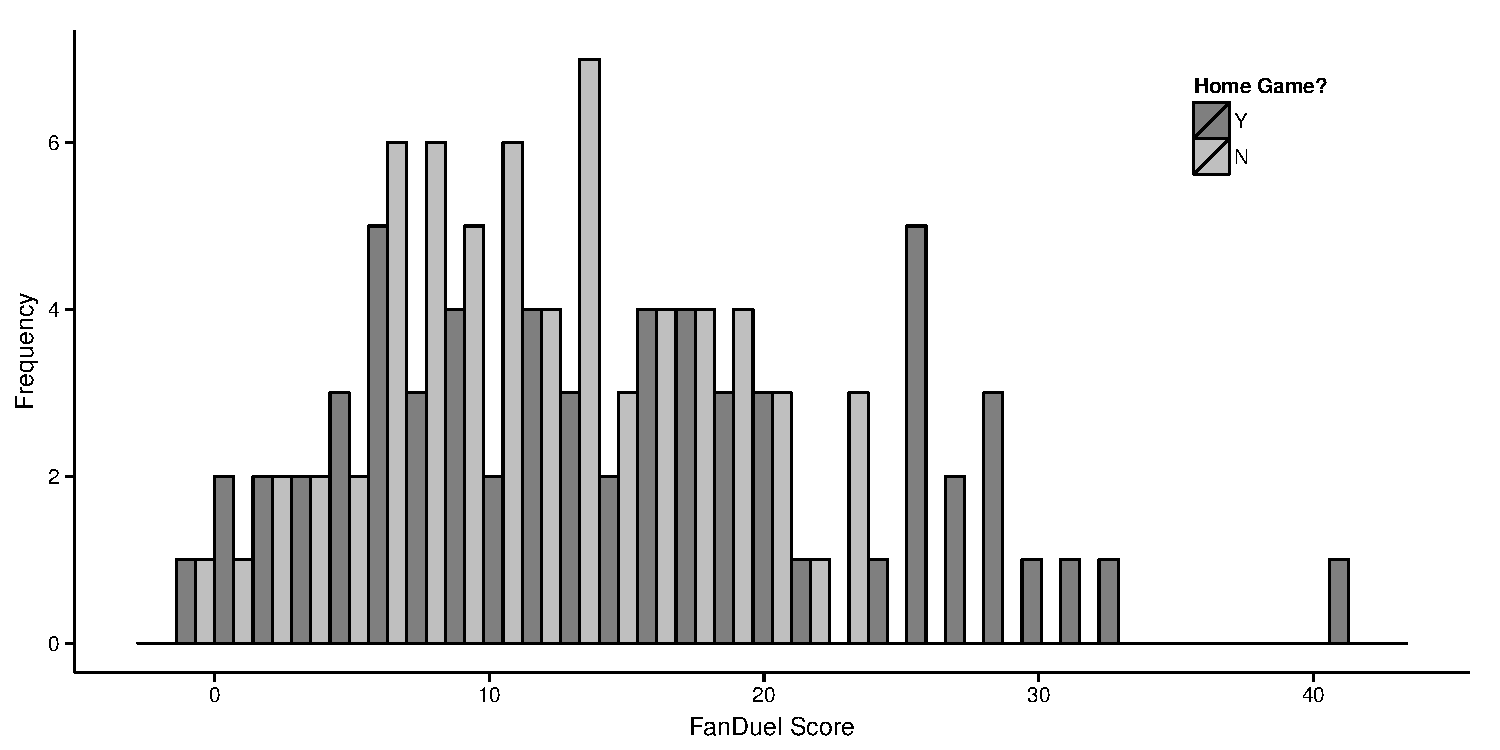
\includegraphics[width=\textwidth]{../figures/beast_mode.pdf}
\end{figure}
%------------------------------------------------------------------------

Figure \ref{beast.mode} shows all of Lynch's past performances through week nine of the 2015 season.  The variability in the performances is presumably due to a variety of factors.  For example, Lynch's top performances all occur during home games.  Other factors might include the strength of the opposing team's defense, Lynch's health, performances by Lynch's teammates, etc.  The sheer number of likely contributors to any one performance is why they are so hard to predict.  

One way to avoid this modeling problem is to just ignore it altogether.  We can simply assume that Lynch's performance during any given game is a random draw from the distribution of his scores shown in Figure \ref{beast.mode}.  In other words, we ignore all the potential contributors and simply assume that the Lynch we observe this week will be one of the Lynch's we observed in some past week.  To be sure this assumption is strong and most likely incorrect.  For instance, if we knew Lynch was not playing at home we should probably throw out all of his performances above 24 points.  However, this starts us down a dangerous path of adding more and more complexity.  Should we throw out games later in the season too?  What if the game was on a Monday instead of a Sunday?  What if the opponent is a division rival?  Such questions continue \emph{ad infinitum}.

Returning to \eqref{f.exp}, we can define a lagged performance as:
\begin{gather}
\hat f_i^L \in \bm{F_i}
\end{gather}
where $F_i^L$ is the set of all past performances by player $i$.  In the case of Lynch, $F_i^L$ contains all the observed performances illustrated by Figure \ref{beast.mode}.  If player $i$ has no past performances we substitute the average weekly performances from across the league at that player's position.  The benefit of this approach is that we can take a draw of past performances for all the players, calculate their expected performances via \eqref{f.exp}, and then solve the problem defined by \eqref{obj} and \eqref{con}.  Repeating this process over and over again generates a frequency distribution that a given team also ends up being optimal among all the samples from the $F_i^L$'s.  If some team -- call it $\bm{x^*} $ -- is optimal sufficiently often than we might expect $\bm{x^*}$ to be robust to winning regardless of the actual realization of $\bm{f}$ (at least in expectation).

\subsection*{Results}

The following analysis illustrates the above method for the limited fantasy game which included:
\[
\begin{array}{rcl}
\text{The Chicago Bears} & \text{@} & \text{The San Diego Chargers} \\
\text{The Buffalo Bills} & \text{@} & \text{The New York Jets} 
\end{array}
\]
The set of available players for the fantasy team was refined from those actually available in each of the above match-ups by eliminating players who were listed as Questionable, Doubtful, Out, or on Injured Reserve.  Players who received a projection of zero on FantasyPro's were also eliminated; this removes backups who were unlikely to play.  For those players that received no projection on FantasyPro's the average projection for their position was used.

A total of 100,000 samples were taken from the $F_i^L$'s.  The linear programming packages \texttt{lpSolve} and \texttt{Rglpk} -- both built for \texttt{R} -- were used to solve the problem defined by \eqref{obj} and \eqref{con}.  Thus, for each of the draws, two solutions were found.  Typically, these solutions were the same but in some cases they differed due to differences in the algorithms used by each of the packages.

%------------------------------------------------------------------------	
\begin{figure}[!t]
\centering
\caption{Frequency distribution of optimal fantasy teams} \label{team.freq}
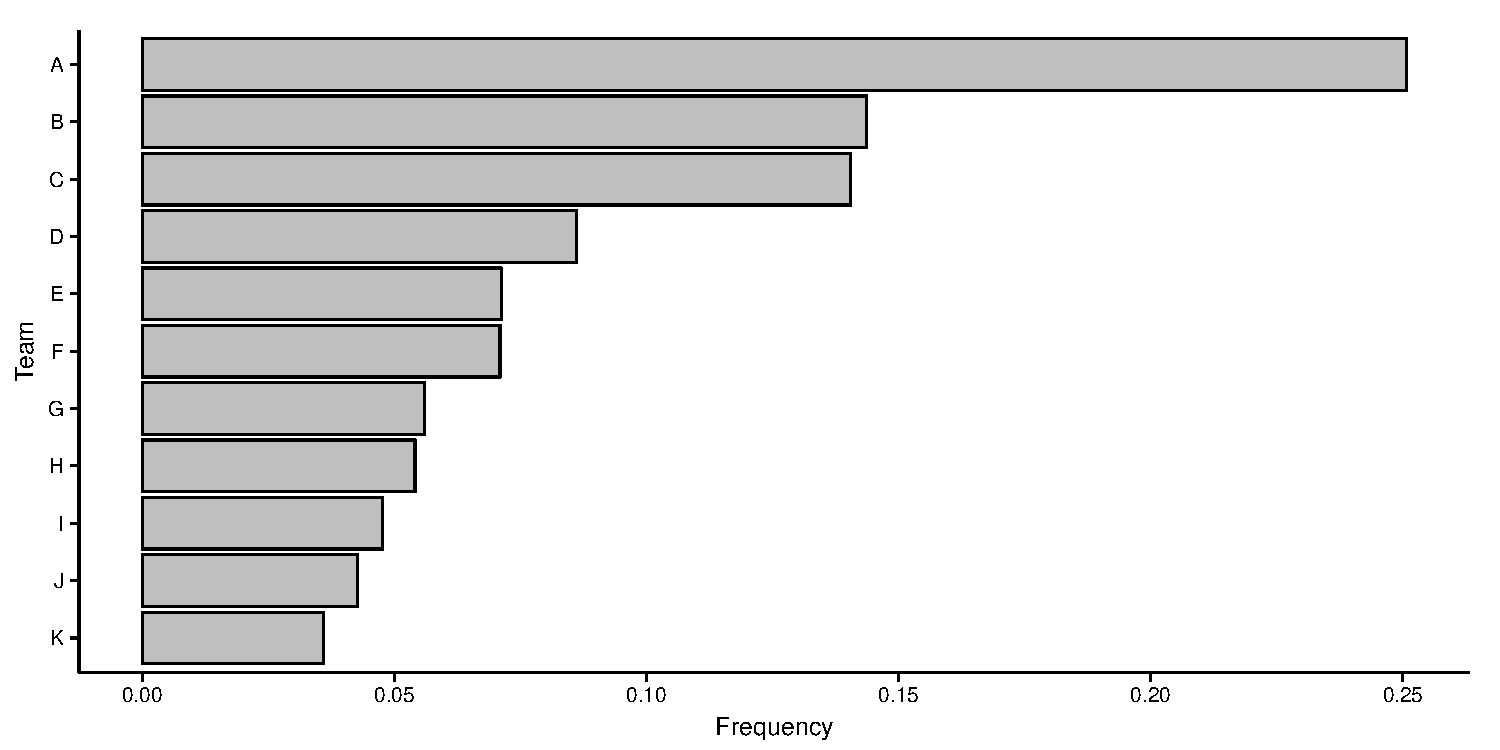
\includegraphics[width=\textwidth]{../figures/team_freq_intro.pdf}
\end{figure}
%------------------------------------------------------------------------

Figure \ref{team.freq} shows the results from applying this resampling method.  Team A consisting of:
\begin{multicols}{3}
\begin{itemize}
	\item Phillip Rivers
	\item Chris Ivory
	\item Danny Woodhead
	\item Alshon Jeffery
	\item Brandon Marshall
	\item Antonio Gates
	\item Eric Decker
	\item Robbie Gould
	\item New York Jets Defense
\end{itemize}
\end{multicols}
\noindent was optimal in just over 25\% of the samples.  Teams B and C were each optimal in roughly 15\% of the samples.  Comparing these to Team A, Teams B and C use Karlos Williams instead of Christopher Ivory or Danny Woodhead and also use the Buffalo Bills Defense instead of the New York Jets Defense.  Clearly, however, a smoking gun was not found; Team A only won 25\% of the time.

%------------------------------------------------------------------------	
\begin{figure}[!t]
\centering
\caption{Frequency distribution of optimal fantasy players} \label{player.freq}
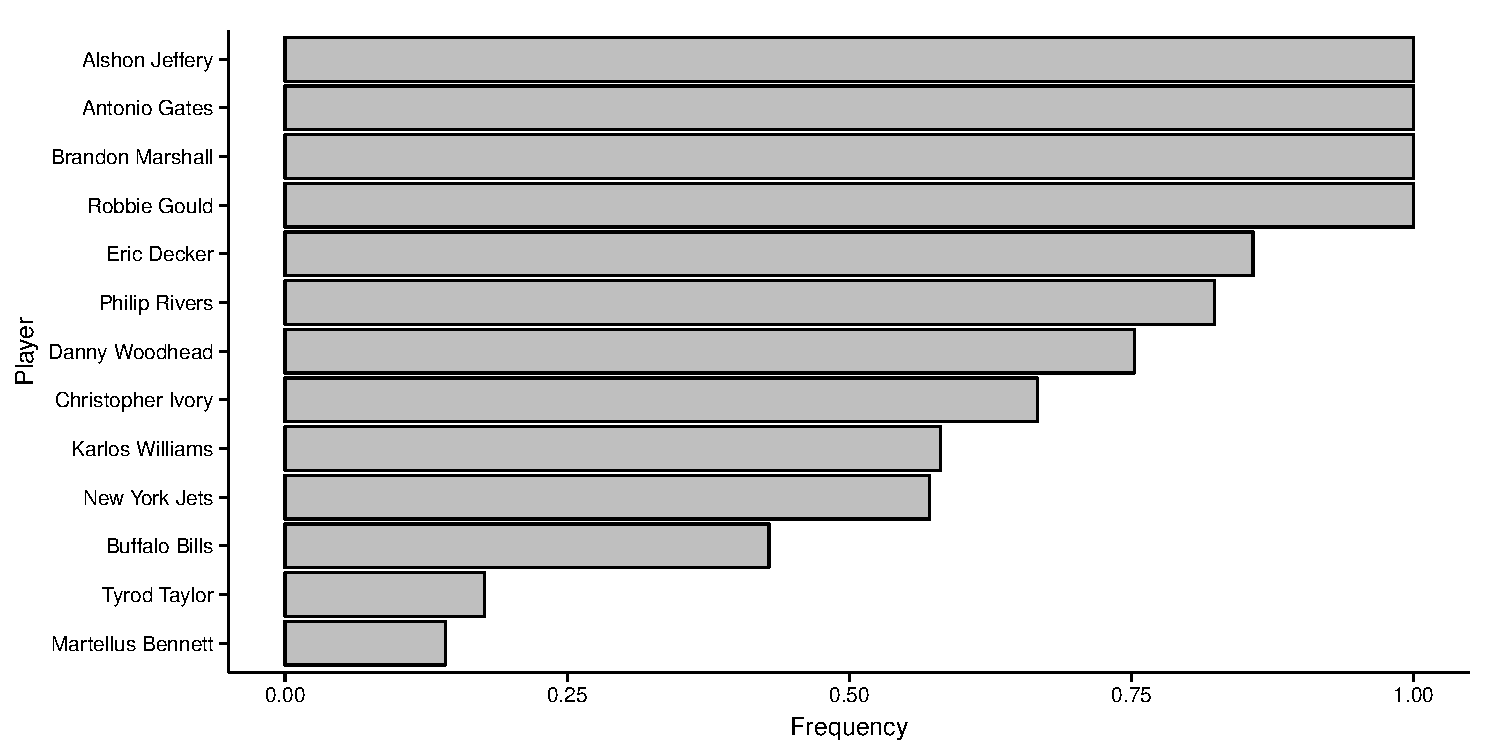
\includegraphics[width=\textwidth]{../figures/player_freq_intro.pdf}
\end{figure}
%------------------------------------------------------------------------

More distressing is the fact that such high team frequencies are much less likely to be seen when considering fantasy games which include all the Sunday and Monday games.  This is simply because there are so many more possible teams.  With this in mind, an additional metric likely to be useful is the frequency of times a certain player is on the optimal team.  Figure \ref{player.freq} illustrates these frequencies.  We can see that Alshon Jeffery, Antonio Gates, Brandon Marshall, and Robbie Gould were members of every winning team.  Furthermore, we could look at frequency plots based on position to better improve player selection.

In fact, a next step might be to iterate over these frequency calculations by treating only those players that appear on the winning in a sufficiently large number of samples as actually available.  We could then choose the optimal team from this smaller set.  This procedure could be repeated until the smallest possible set of players is found that can still generate an ``eligible" and affordable team.  The optimal team from this smallest set could then serve as our prediction.

\end{document} 